\documentclass[11pt]{article}
\usepackage[top=2.8cm, bottom=2.8cm, left=2cm, right=2cm]{geometry}
\usepackage{hyperref}
\usepackage{algorithm2e}
\usepackage[numbers]{natbib}
\bibliographystyle{plainnat}
\usepackage{appendix}
\usepackage[table]{xcolor}
\usepackage{pgfplots}
\usepackage{pgfplotstable}
\usepackage[font={color=darkgray,footnotesize, sf, it}]{caption}
\usepackage{amsmath}
\usepackage{helvet}
\usepackage{wrapfig}
\usepackage[eulergreek]{sansmath}
\usepackage{listings}
\usepackage{setspace}
\usepackage{graphicx}
\usepackage{longtable}
\usepackage{minted}
\usepackage{relsize}
\linespread{1.2}
\lstset { %
    language=C++,
    backgroundcolor=\color{black!5}, % set backgroundcolor
    basicstyle=\ttfamily\footnotesize,% basic font setting
}
\usepackage{bchart}
\usepackage{booktabs}
\usepackage{xcolor}

\lstdefinestyle{BashInputStyle}{
  language=bash,
  basicstyle=\footnotesize\ttfamily,
  numbers=left,
  numberstyle=\tiny,
  numbersep=3pt,
  frame=tb,
  columns=fullflexible,
  backgroundcolor=\color{cyan!20},
  linewidth=0.95\linewidth,
  xleftmargin=0.1\linewidth
}

\definecolor{skyblue}{RGB}{203,240,255}
\definecolor{forestgreen}{RGB}{0,96,50}
\definecolor{indigo}{RGB}{4,87,239}
\definecolor{darkindigo}{RGB}{1,40,112}
\definecolor{darkpurple}{RGB}{32,14,104}
\definecolor{apple}{RGB}{0,158,13}
\definecolor{bad}{RGB}{239,55,55}
\definecolor{badtoavg}{RGB}{247,128,98}
\definecolor{avg}{RGB}{255,218,117}
\definecolor{avgtogood}{RGB}{190,247,140}
\definecolor{good}{RGB}{102,226,102}

\setlength{\parindent}{0em}
\setlength{\parskip}{1em}
\setlength\parindent{0pt}

\usepackage{tikz}
\usepackage{collcell}
\usetikzlibrary{shapes.geometric, arrows,calc}
\tikzstyle{startstop} = [rectangle, font=\small, rounded corners, minimum width=4cm, minimum height=0.8cm,text centered, text width=4.5cm, draw=black, fill=gray!50]
\tikzstyle{barrier} = [rectangle, font=\small, rounded corners, minimum width=4cm, minimum height=0.8cm,text centered, text width=4.5cm, draw=black, fill=red!50]
\tikzstyle{mainproc} = [rectangle, font=\small, minimum width=5cm, minimum height=0.8cm, text centered, text width=5cm, draw=black, fill=cyan!50]
\tikzstyle{threadproc} = [rectangle, font=\small, minimum width=4.5cm, minimum height=0.8cm, text centered, text width=4.5cm, draw=black, fill=orange!70]
\tikzstyle{decision} = [diamond, font=\small, align=center, minimum height=4ex, diamond, aspect=2, text width=14em, inner sep=-1pt, draw=black, fill=violet!50]
\tikzstyle{arrow} = [thick,->,>=stealth]
\tikzstyle{line} = [draw, -latex']

\usepackage{titlesec}

\titlespacing\section{0pt}{12pt plus 4pt minus 2pt}{0pt plus 2pt minus 2pt}
\titlespacing\subsection{0pt}{12pt plus 4pt minus 2pt}{0pt plus 2pt minus 2pt}
\titlespacing\subsubsection{0pt}{12pt plus 4pt minus 2pt}{0pt plus 2pt minus 2pt}

\date{}
\author{}
\title{{\color{indigo}\textbf{CM30225: Parallel Computing}}\\\small \textbf{Shared Memory Architectures: Balena, pthreads and C\\November 2018}\vspace{-15ex}}
\SetKwInOut{Parameter}{parameter}

\begin{document}
\maketitle
\footnotesize\tableofcontents
\clearpage
\normalsize
\pgfplotsset{compat=1.16}

{\color{indigo}
\section{Introduction}}
A \textit{``multiprocessor architecture''} is a broad term applied to parallel architectures involving more than one full processor. A shared memory architecture is an approach to multiprocessor design which relies on a set of $\mathcal{N}$ processors, each connected via a shared memory bus to main memory. Access to memory is substantially slower than processor speeds, as all accesses must go through the shared bus which is the quintessential bottleneck in the design. Changes to values stored in shared memory are globally visible and access to shared values is incredibly slow when more than one processor wishes to perform an update \cite{elrewini2005}. For this reason, shared memory architectures are generally appropriate for small-scale implementations (less than 100 cores).  Programmers must consider carefully the use of shared variables in programs which will reside in main memory. In order to combat slow memory accesses via the bus, processors will usually keep a cached copy of shared data, which introduces the cache coherency problem - maintaining consistent and updated copies of values in shared main memory is very difficult when values can be modified in any order by other processors \cite{goodman1983}. This assignment requires consideration of the above in implementing matrix relaxation using a shared memory architecture.

{\color{darkindigo}
\subsection*{Matrix Relaxation}}
Matrix relaxation involves repeatedly replacing a cell's value with the average of its four neighbours (excepting boundary values) until values settle down to a given precision. The task in question was to use C and the POSIX library to implement relaxation on a square matrix of dimension $d$, using $t$ threads\footnote{The number of \texttt{pthread} threads created, not including the program's main thread.} to a precision of $p$.  The solution was run on \textsl{Balena}, the High Performance Cluster (HPC) at University of Bath\footnote{\url{https://www.bath.ac.uk/corporate-information/balena-hpc-cluster/}} using a variety of configurations to investigate the scalability and correctness of the parallel approach on various problem sizes.  Matrix relaxation holds some inherent sequential properties which require careful synchronisation between threads, as the order of computations is crucial to the output:
\begin{enumerate}
\item \textbf{Consistency of neighbour cells:} For any \textit{inner cell} $c_{i,j}$ (where $i$ is the row and $j$ is the column) to be correctly relaxed, the neighbouring cells ($c_{i+1,j}$, $c_{i-1,j}$, $c_{i,j+1}$, $c_{i,j-1}$) must be kept consistent values throughout the iteration. If any neighbouring cell values were changed (or \textit{relaxed}) between reads for a certain cell, this would cause the value of the cells in the resulting matrix to be incorrect and unpredictable between iterations.  The matrix needs to be divided in such a way without interfering with other threads' computations.
\item \textbf{Precision checks between iterations:} Before a new iteration can start, there needs to be a check across all inner cells as to whether the difference in corresponding matrix values before and after the current iteration is less than or equal to the chosen precision, $p$. There must be careful management over when computation can proceed as threads are very unlikely to be in lockstep.
\end{enumerate}

{\color{indigo} 
\section{Sequential Approach}
\label{sec:seqapproach}}
As in Algorithm \ref{alg:relaxationsequential}, the sequential approach relied on working with two matrices of the same dimension $d$ and swapping the references to these after each iteration. This way, the output matrix of iteration $i$ becomes the input to iteration $(i+1)$.  The problem of neighbour cell inconsistency discussed previously is avoided with the introduction of this second (output) matrix. This comes at the cost of an increase in space complexity in memory on the heap, but this is still linear in $d$ which is an appropriate trade off in order to avoid incorrect calculations (new space complexity is $O(2d) = O(d)$, where $d$ is the dimension of the matrix). The fact that swapping input and output matrices comes at the end of each iteration means that no cell can be overwritten with a new relaxed value until every other cell's relaxed value has already been calculated. At step \texttt{9} of Algorithm \ref{alg:relaxationsequential} there is a potentially expensive operation in swapping matrices between every iteration. In order to reduce this overhead, the implementation instead swaps the \textit{references} to each matrix, not the values of each and every inner cell. 

\RestyleAlgo{algoruled}
\LinesNumbered
\DontPrintSemicolon
\SetAlgoLined
\colorbox[gray]{0.95}{
\begin{minipage}{\textwidth}
\begin{algorithm}[H]
  	\caption{Matrix relaxation (sequential).\label{alg:relaxationsequential}}
  	{\color{darkgray}\KwIn{A $d \times d$ matrix with equal fixed edge values and chosen inner values.}
	\KwOut{A $d \times d$ matrix with equal fixed edge values and \textit{\textbf{relaxed}} inner values.}
	\KwData{$d$: Dimension of matrix, $p$: Precision
	}}
	\BlankLine
	{\color{darkgray}Extract program arguments\;
 	Create matrices \texttt{matA} and \texttt{matB} of dimension $d$\;
 	Initialise \texttt{matA} and \texttt{matB} with identical contents\;
 	\BlankLine
 	\Repeat{\texttt{abs(matB[i][j] - matA[i][j])} $\leq p$ for all $(i,j)$}{
		\BlankLine
		\ForEach{inner cell $(i,j)$}
			{\texttt{total $=$ matA[i+1][j]$+$matA[i-1][j]$+$matA[i][j+1]$+$matA[i][j-1]\; matB[i][j] $=$ total $\div$ 4\;}}
 		\BlankLine
 		Swap \texttt{matA} and \texttt{matB}\;
 		}}
\end{algorithm}
\end{minipage}}
\normalsize

\newpage
{\color{indigo}
\section{Parallel Approach}
\label{sec:parapproach}}
As with any algorithm, attempting to run operations in parallel brings initial overheads in the form of:
\begin{enumerate}
\item \textbf{Management of threads:} Creation, joining and destroying \texttt{pthreads} is an overhead \cite{anderson1989} which was minimised by adopting a \textit{``thread pool''} design, which fixes this overhead to once during the program lifetime \cite{syer2011}. Threads are re-used every iteration and destroyed together once precision is reached. If this was done on every iteration the overhead would be substantial (e.g. when $p$ is small, and starting values are a large distance from the converged result causing lots of iterations).
\item \textbf{Management of data:} Allocating each thread a certain number of cells to relax in parallel is another overhead. When the problem size is very small this overhead is relatively large, but when the value of $d$ increases this relative cost is reduced. Larger problem sizes (bigger matrices) should reasonably render this initial overhead small compared to the total runtime.
\end{enumerate}

Algorithm \ref{alg:relaxationparallel} describes the parallel approach, which also uses two matrices of dimension $d$, initialised with identical values. The matrix is divided evenly as possible between threads so that cells can be relaxed in parallel. Once each thread has finished working on the number of cells it has been assigned, there is synchronisation across threads in order to check if another iteration is needed.
\\
\RestyleAlgo{algoruled}
\LinesNumbered
\DontPrintSemicolon
\SetAlgoLined
\colorbox[gray]{0.95}{
\begin{minipage}{\textwidth}
\begin{algorithm}[H]
  	\caption{Matrix relaxation (parallel).\label{alg:relaxationparallel}}
  	{\color{darkgray}\KwIn{A $d \times d$ matrix with equal fixed edge values and chosen inner values.}
				\KwOut{A $d \times d$ matrix with equal fixed edge values and \textit{\textbf{relaxed}} inner values.}
				\KwData{$d$: Dimension of matrix, $p$: Precision, $t$: Number of threads}}
	\BlankLine
	{\color{darkgray}Extract program arguments\;
 	Create matrices \texttt{matA} and \texttt{matB} of dimension $d$\;
 	Initialise \texttt{matA} and \texttt{matB} with identical contents\;
 	Distribute $(d-2)^2$ inner cells of \texttt{matA} and \texttt{matB} between $t$ threads\;
	Create and start $t$ threads to relax assigned cells\;
	\Repeat{\texttt{abs(matB[i][j] - matA[i][j])} $\leq p$ for all $(i,j)$ across $t$ threads}{
		\BlankLine
		\ForEach{inner cell $(i,j)$ assigned to each thread}
			{\texttt{total $=$ matA[i+1][j]$+$matA[i-1][j]$+$matA[i][j+1]$+$matA[i][j-1]\; matB[i][j] $=$ total $\div$ 4\;}}
 		\BlankLine
 		Synchronise $t$ threads\;
		\If{\texttt{abs(matB[i][j] - matA[i][j])} $> p$ for any $(i,j)$ across $t$ threads}{Swap \texttt{matA} and \texttt{matB}\; }
 		}}
\end{algorithm}
\end{minipage}}

{\color{darkindigo}
\subsection*{Choice of Concurrency Primitives}}
Out of several choices of concurrency primitives (e.g. barriers, mutexes, semaphores, condition variables), the use of \texttt{pthread\_barrier\_t} barriers was adopted to synchronise computations across several threads, ensuring $t$ threads had finished an iteration before precision values were calculated. Other primitives were considered but decided inappropriate for this task. Mutexes alone would provide mutual exclusion in accessing critical regions but not synchronization, and (although a candidate for synchronisation) condition variables have been subject to the problem of spurious ``wake-ups'' \cite{butenhof1997}. Use of semaphores is primarily appropriate in problems synchronising two threads rather than many, with the counting semaphores approach requiring a lot of inter-thread communication to signal and wait for when resources are available.  Barriers require the least amount of code on the programmer's behalf in getting a specific number threads to wait for all to reach a certain stage in a computation before they can continue.  Without barriers between iterations there would be race conditions and unpredictable results in computations \cite{brawer1989}, as matrix relaxation is an example of a problem where the calculated solution can be dependent on the execution speed of each thread if no synchronisation primitives are adopted. For these reasons, barriers were chosen as a suitable concurrency primitive for the problem.

{\color{darkindigo}
\subsection*{Avoiding Race Conditions}}
A race condition is defined as the consequence of multiple threads reading and writing a shared value with the final result of operations dependent on the order of execution \cite{carr2002}. A data race is a type of race condition which occurs when two or more threads access a shared location and at least one access is a write which is not enforced using synchronization primitives \cite{kasikci2012}. In the parallel implementation, both of these situations are avoided using the below strategy.

Each process has a reference 


keeps a reference to the input and output matrices but only updates the values of the cells in the output matrix that it has been assigned. All threads are prevented from continuing to the next iteration using barriers, as described above. Critically, this approach means there is no need to use locks to protect access to the elements of either matrix. During a single iteration on any thread:
\begin{itemize}
\item Each element of the first (input) matrix can be read from any number of times without worrying about other threads updating any of its elements. 
\item Each element of the second (output) matrix is written to once per iteration. There is no potential for simultaneous read or write operations on the same element of the output matrix.
\item Calculating the precision (difference between corresponding cells) is a read-only operation.
\item Threads swap their references to input and output matrices and a precision check across all threads is done in a synchronised fashion. No thread starts a new iteration before the previous one has finished.
\end{itemize}

{\color{darkindigo}
\subsection*{Dividing the Task Between Threads}}
Due to the ``unfair'' and unpredictable nature in which threads are scheduled and executed by the OS, I decided to split the number of cells to relax equally as possible between threads. Otherwise, if a single thread was given the bulk of the cells to relax and was de-scheduled by the OS in favour of a thread with less cells to relax, it may produce an overall execution time that is larger. This uneven split would cause runtime to vary drastically based on how the OS decides to schedule threads. Instead of relying on a ``lucky'' scheduling of tasks by the OS, the total number of cells was instead spread as evenly as possible so that the total runtime per thread should not vary significantly. For a $d \times d$ matrix, there are $(d-2)^{2}$ inner cells which need relaxing. It follows that by splitting the cells as equally as possible across $t$ threads, then each thread should receive $(d-2)^{2} \div t$ cells to relax. As this is just integer division, it may mean the number of cells does not divide exactly by the number of threads. If there is any remainder, this is given by $(d-2)^{2} \mod t$. In keeping with the approach of an even distribution of cells across threads, this remainder is spread across threads in an even fashion too, to balance workload. 

Once all cells have been divided across threads, the important single call to \texttt{pthread\_create} can be made for each thread, passing in data to the \texttt{submatrix\_relax} function where threads can start relaxing their part of the matrix.

{\color{darkindigo}
\subsection*{Precision Checks}}
In order to determine when relaxation has finished across all threads, a global boolean flag called \texttt{all\_within\_precision} is used, along with a global boolean array of size equal to $t$, the number of threads (called \texttt{next\_iteration\_needed}). Each thread is responsible for updating its slot in the global \texttt{next\_iteration\_needed} array, indicating to the main thread whether the precision is reached for all cells allocated to that thread. I did initially consider use of a lock and counter variable to check how many threads had finished, however a simpler solution existed which was less costly in terms of runtime than maintaining locks around critical regions.  Use of \texttt{pthread\_barrier\_t} barriers allows for synchronisation across multiple threads between iterations, in a ``superstep'' approach (as shown in Figure \ref{fig:superstep}). As the purpose of the calls to \texttt{pthread\_barrier\_wait} is to create a synchronisation point where all threads must hit before they can continue, it was important to minimise the necessary work between each barrier call so that each thread could do as much work in parallel as possible. As such, each thread is not just responsible for relaxing the cells it has been assigned, but also calculating the precision. 

\begin{figure}[H]
\centering
\includegraphics[scale=0.25]{img/superstep.png} 
\caption{Diagram showing the ``superstep programming'' method with barriers.}\label{fig:superstep}
\end{figure}

If the precision for thread $n$ is within the desired range, it updates its dedicated element in the global array - \texttt{next\_iteration\_needed[n]}. As all threads have a dedicated element in this array, it means that no data races occur for overwriting the same element in the array, preventing the need for locks around any regions including array updates. It also means that the work to compute precision is divided by $t$, the number of threads instead of giving the main thread $(d-2)^{2}$ cells to compute precision for in between \texttt{pthread\_barrier\_wait} calls.  The only work that the main thread does between barrier calls is to check if any values in the \texttt{next\_iteration\_needed} array are set to \texttt{true}. If this is the case, the global flag \texttt{all\_within\_precision} that each thread checks for after an iteration is set to \texttt{false} and threads move to the next iteration, swapping their references to the input and output matrices. It is important that the main thread sets this flag before the second barrier is hit, ensuring all threads read the updated value before deciding if a new iteration is necessary. Eventually after a certain number of iterations it may be that all values in the \texttt{next\_iteration\_needed} array are set to \texttt{false}. When this happens, the matrix has been relaxed to the desired precision across all $t$ threads, which means the single call to \texttt{pthread\_join} can be made for each thread to terminate and join the main thread before the relaxed matrix is displayed. \textbf{Figures \ref{fig:main} and \ref{fig:workers} show both the main thread and \texttt{pthread} flow of control.}
\\
\normalsize
\begin{figure}[H]
	\begin{minipage}{0.47\textwidth}
       \hspace{-0.2cm}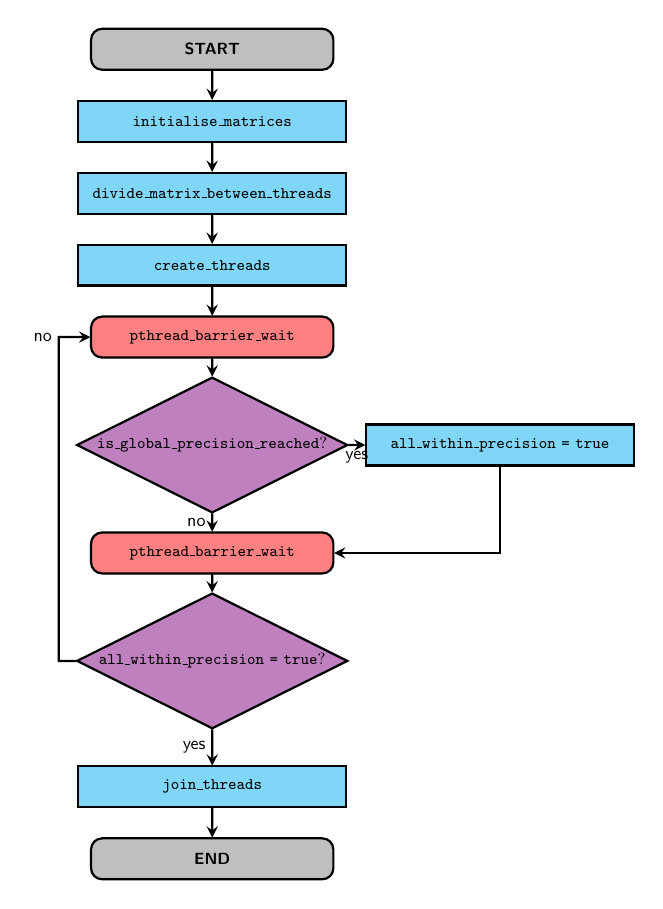
\begin{tikzpicture}[node distance=4em,thick,scale=0.65, every node/.style={scale=0.65}]
\node (start) [startstop] {\textsf{\textbf{START}}};
\node (initMat) [mainproc, below of=start] {\texttt{initialise\_matrices}};
\node (divideMat) [mainproc, below of=initMat] {\texttt{divide\_matrix\_between\_threads}};
\node (createThreads) [mainproc, below of=divideMat] {\texttt{create\_threads}};
\node (barrier1) [barrier, below of=createThreads] {\texttt{pthread\_barrier\_wait}};
\node (precCheck) [decision, below of=barrier1, yshift=-2em] {\texttt{is\_global\_precision\_reached}?};
\node (setFlag)  [mainproc, right of=precCheck, xshift=12em] {\texttt{all\_within\_precision = true}};
\node (barrier2) [barrier, below of=precCheck, yshift=-2em] {\texttt{pthread\_barrier\_wait}};
\node (globalDone) [decision, below of=barrier2, yshift=-2em] {\texttt{all\_within\_precision = true}?};
\node (joinThreads) [mainproc, below of=globalDone, yshift=-3em] {\texttt{join\_threads}};
\node (end) [startstop, below of=joinThreads] {\textsf{\textbf{END}}};

\draw [arrow] (start) -- (initMat);
\draw [arrow] (initMat) -- (divideMat);
\draw [arrow] (divideMat) -- (createThreads);
\draw [arrow] (createThreads) -- (barrier1);
\draw [arrow] (barrier1) -- (precCheck);
\draw [arrow] (barrier2) -- (globalDone);
\draw [arrow] (joinThreads) -- (end);
\draw [arrow] (precCheck) -- node[anchor=north] {\textsf{yes}} (setFlag);
\draw [arrow] (precCheck) -- node[anchor=east] {\textsf{no}} (barrier2);
\draw [arrow] (setFlag) |- (barrier2);
\draw [arrow] (globalDone) -- node[anchor=east] {\textsf{yes}} (joinThreads);
\draw [arrow] (globalDone) -- ++(-3,0) |- node[anchor=east] {\textsf{no}} (barrier1);
\end{tikzpicture}
        \caption{Diagram of the main thread execution life cycle.}
        \label{fig:main}
    \end{minipage}\hspace{0.3cm}\vline\hspace{1.1cm}
    \begin{minipage}{.47\textwidth}
        \hspace{-1cm}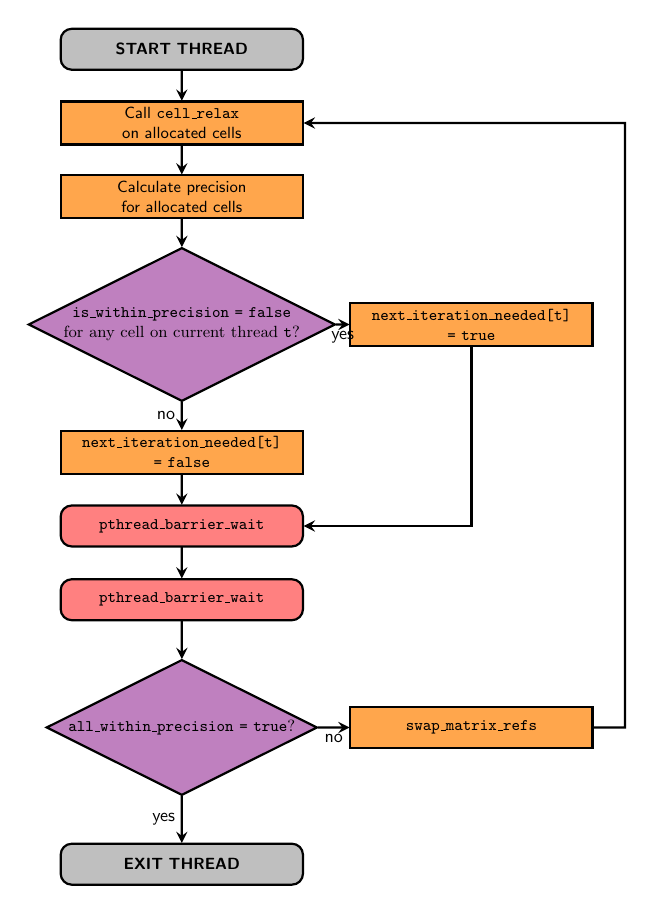
\begin{tikzpicture}[node distance=4.1em,thick,scale=0.65, every node/.style={scale=0.65}]
\node (start) [startstop] {\textsf{\textbf{START THREAD}}};
\node (relax) [threadproc, below of=start] {\textsf{Call} \texttt{cell\_relax} \textsf{on allocated cells}};
\node (calcPrec) [threadproc, below of=relax] {\textsf{Calculate precision for allocated cells}};
\node (precCheck) [decision, below of=calcPrec, yshift=-3em] {\texttt{is\_within\_precision = false} for any cell on current thread \texttt{t}?};
\node (setFlagTrue)  [threadproc, right of=precCheck, xshift=12em] {\texttt{next\_iteration\_needed[t] = true}};
\node (setFlagFalse)  [threadproc, below of=precCheck, yshift=-3em] {\texttt{next\_iteration\_needed[t] = false}};
\node (barrier1) [barrier, below of=setFlagFalse] {\texttt{pthread\_barrier\_wait}};
\node (barrier2) [barrier, below of=barrier1] {\texttt{pthread\_barrier\_wait}};
\node (globalDone) [decision, below of=barrier2, yshift=-3em] {\texttt{all\_within\_precision = true}?};
\node (swapArrays)  [threadproc, right of=globalDone, xshift=12em] {\texttt{swap\_matrix\_refs}};
\node (end) [startstop, below of=globalDone, yshift=-3.5em] {\textsf{\textbf{EXIT THREAD}}};

\draw [arrow] (start) -- (relax);
\draw [arrow] (relax) -- (calcPrec);
\draw [arrow] (calcPrec) -- (precCheck);
\draw [arrow] (precCheck) -- node[anchor=east] {\textsf{no}} (setFlagFalse);
\draw [arrow] (precCheck) -- node[anchor=north] {\textsf{yes}} (setFlagTrue);
\draw [arrow] (setFlagTrue) |- (barrier1);
\draw [arrow] (setFlagFalse) -- (barrier1);
\draw [arrow] (barrier1) -- (barrier2);
\draw [arrow] (barrier2) -- (globalDone);
\draw [arrow] (globalDone) -- node[anchor=north] {\textsf{no}} (swapArrays);
\draw [arrow] (globalDone) -- node[anchor=east] {\textsf{yes}} (end);
\draw [arrow] (swapArrays) -- ++(3,0) |- (relax);
\end{tikzpicture}
        \caption{Diagram of the \texttt{pthread} execution life cycle.}
        \label{fig:workers}
    \end{minipage}
\end{figure}

{\color{indigo}
\section{Testing Program Correctness}}
In order to verify whether the approach taken was correct, it required a combination of manual verification and a set of varied test cases, where input and output were compared for correctness. See Appendix \ref{apdx:runprog} for how to run the parallel implementation with different configurations.

{\color{darkindigo}
\subsection*{Manual Verification}}
The first stage in testing program correctness was to check against a manually-calculated matrix relaxation in order to check that the parallel C implementation finished after an equal number of iterations and contained equal cell values to the manually-calculated relaxed matrix. The relaxation process was executed by hand on the below $5 \times 5$ matrix using the following arguments: $d = 5$, $p = 0.2$, $t = 3$.  Using the parallel algorithm shown in Algorithm \ref{alg:relaxationparallel}, the $(d-2)^{2} = 9$ inner cells are divided equally across the 3 threads, as shown in Table \ref{tbl:cellbreakdown}. Between iterations, the maximum difference in cell values ($\max(|c_{new}-c_{old}|)$) for each thread was calculated, to check if this was within the desired precision of $p = 0.2$. \textbf{Rows and columns are indexed from 0.} 

\begin{table}[h]
\begin{center}
\caption{Inner cell breakdown for $d = 5$, $t = 3$.}
\label{tbl:cellbreakdown}
\begin{tabular}{|c|c|}
\hline
\textbf{Thread} & \textbf{Inner cells to relax} \\
\hline
\texttt{1} & $(1,1), (1,2), (1,3)$\\
\texttt{2} & $(2,1), (2,2), (2,3)$\\
\texttt{3} & $(3,1), (3,2), (3,3)$\\
\hline
\end{tabular}
\end{center}
\end{table}

The manual calculation was as follows:

\hspace{-0.2cm}\begin{minipage}{0.47\textwidth}
$
\begin{bmatrix}
1.000000 & 1.000000 & 1.000000 & 1.000000 & 1.000000 \\
1.000000 & 0.001251 & 0.563585 & 0.193304 & 1.000000 \\
1.000000 & 0.808741 & 0.585009 & 0.479873 & 1.000000 \\
1.000000 & 0.350291 & 0.895962 & 0.822840 & 1.000000 \\
1.000000 & 1.000000 & 1.000000 & 1.000000 & 1.000000 \\
\end{bmatrix}
$
\end{minipage}\hspace{1.8cm}{\color{cyan!90}\vline}\hspace{0.5cm}
\begin{minipage}{.47\textwidth}
\vspace{-1em}
\textbf{Initial Matrix:} The matrix of \texttt{double} values is set to $1.000000$ on the edges, and random values between 0 and 1 on the inner cells.
\vspace{-1em}
\end{minipage}

\hspace{-0.2cm}\begin{minipage}{0.47\textwidth}
$
\begin{bmatrix}
1.000000 & 1.000000 & 1.000000 & 1.000000 & 1.000000 \\
1.000000 & 0.843081 & 0.444891 & 0.760865 & 1.000000 \\
1.000000 & 0.484138 & 0.687040 & 0.650288 & 1.000000 \\
1.000000 & 0.926176 & 0.689535 & 0.843959 & 1.000000 \\
1.000000 & 1.000000 & 1.000000 & 1.000000 & 1.000000 \\
\end{bmatrix}
$
\end{minipage}\hspace{1.8cm}{\color{cyan!90}\vline}\hspace{0.5cm}
\begin{minipage}{.47\textwidth}\textbf{Iteration 1:}\\
\\
\begin{tabular}{|c|c|c|}
\hline
\textbf{Thread} & \textbf{$\max(|c_{new}-c_{old}|)$} & \textbf{$\leq p$?} \\
\hline
\texttt{1} & $|0.843081-0.001251|$ & {\color{red}\texttt{false}}\\
\texttt{2} & $|0.484138-0.808741|$ & {\color{red}\texttt{false}}\\
\texttt{3} & $|0.926176-0.350291|$ & {\color{red}\texttt{false}}\\
\hline
\end{tabular}
\end{minipage}

\hspace{-0.4cm}\begin{minipage}{0.47\textwidth}
$
\begin{bmatrix}
1.000000 & 1.000000 & 1.000000 & 1.000000 & 1.000000 \\
1.000000 & 0.732257 & 0.822747 & 0.773795 & 1.000000 \\
1.000000 & 0.864074 & 0.567213 & 0.822966 & 1.000000 \\
1.000000 & 0.793418 & 0.864294 & 0.834956 & 1.000000 \\
1.000000 & 1.000000 & 1.000000 & 1.000000 & 1.000000 \\
\end{bmatrix}
$
\end{minipage}\hspace{1.8cm}{\color{cyan!90}\vline}\hspace{0.5cm}
\begin{minipage}{.47\textwidth}\textbf{Iteration 2:}\\
\\
\begin{tabular}{|c|c|c|}
\hline
\textbf{Thread} & \textbf{$\max(|c_{new}-c_{old}|)$} & \textbf{$\leq p$?} \\
\hline
\texttt{1} & $|0.822747-0.444891|$ & {\color{red}\texttt{false}}\\
\texttt{2} & $|0.864074-0.484138|$ & {\color{red}\texttt{false}}\\
\texttt{3} & $|0.864294-0.689535|$ & {\color{blue}\texttt{true}}\\
\hline
\end{tabular}
\end{minipage}

\hspace{-0.4cm}\begin{minipage}{0.47\textwidth}
$
\begin{bmatrix}
1.000000 & 1.000000 & 1.000000 & 1.000000 & 1.000000 \\
1.000000 & 0.921705 & 0.768316 & 0.911428 & 1.000000 \\
1.000000 & 0.773222 & 0.843520 & 0.793991 & 1.000000 \\
1.000000 & 0.932092 & 0.798897 & 0.921815 & 1.000000 \\
1.000000 & 1.000000 & 1.000000 & 1.000000 & 1.000000 \\
\end{bmatrix}
$
\end{minipage}\hspace{1.8cm}{\color{cyan!90}\vline}\hspace{0.5cm}
\begin{minipage}{.47\textwidth}\textbf{Iteration 3:}\\
\\
\begin{tabular}{|c|c|c|}
\hline
\textbf{Thread} & \textbf{$\max(|c_{new}-c_{old}|)$} & \textbf{$\leq p$?} \\
\hline
\texttt{1} & $|0.921705-0.732257|$ & {\color{blue}\texttt{true}}\\
\texttt{2} & $|0.843520-0.567213|$ & {\color{red}\texttt{false}}\\
\texttt{3} & $|0.932092-0.793418|$ & {\color{blue}\texttt{true}}\\
\hline
\end{tabular}
\end{minipage}

\hspace{-0.4cm}\begin{minipage}{0.47\textwidth}
$
\begin{bmatrix}
1.000000 & 1.000000 & 1.000000 & 1.000000 & 1.000000 \\
1.000000 & 0.885385 & 0.919163 & 0.890577 & 1.000000 \\
1.000000 & 0.924329 & 0.783607 & 0.919191 & 1.000000 \\
1.000000 & 0.893030 & 0.924357 & 0.898222 & 1.000000 \\
1.000000 & 1.000000 & 1.000000 & 1.000000 & 1.000000 \\
\end{bmatrix}
$
\end{minipage}\hspace{1.8cm}{\color{cyan!90}\vline}\hspace{0.5cm}
\begin{minipage}{.47\textwidth}\textbf{Relaxed Matrix (4 iterations):}\\
\\
\begin{tabular}{|c|c|c|}
\hline
\textbf{Thread} & \textbf{$\max(|c_{new}-c_{old}|)$} & \textbf{$\leq p$?} \\
\hline
\texttt{1} & $|0.919163-0.768316|$ & {\color{blue}\texttt{true}}\\
\texttt{2} & $|0.924329-0.773222|$ & {\color{blue}\texttt{true}}\\
\texttt{3} & $|0.924357-0.798897|$ & {\color{blue}\texttt{true}}\\
\hline
\end{tabular}
\end{minipage}

This step-by-step manual calculation shows checks for precision across each thread's cells after they have been relaxed, which is used to decide whether another iteration is needed.  Once the manual calculation had taken place, I created a C function to populate the initial matrix with identical values and ran the program to compare outputs:
\begin{lstlisting}[style=BashInputStyle]
    $		./sharedrelax -d 5 -t 3 -p 0.2 -v
\end{lstlisting}
The resulting output included:
\begin{lstlisting}[style=BashInputStyle]
	INFO: ___Relaxed Matrix (4 iterations)_______
	1.000000 1.000000 1.000000 1.000000 1.000000 
	1.000000 0.885385 0.919163 0.890577 1.000000 
	1.000000 0.924329 0.783607 0.919191 1.000000 
	1.000000 0.893030 0.924357 0.898222 1.000000 
	1.000000 1.000000 1.000000 1.000000 1.000000 
\end{lstlisting}

Upon observing that that the parallel C implementation matched the manual example at each step, I varied the value of $t$ from 1 to 9 (the maximum value of $t$ possible for a matrix of this size). Outputs from these tests were saved to files and compared using the Unix \texttt{diff} tool to verify that the total number of iterations required and the matrix values at each stage were identical, which was a success. These outputs are visible in the \texttt{tests} directory of this submission. The manual verification stage was then performed on a variety of other small ($d\leq 6, t\leq 5$) examples, with values compared to the result of the sequential and parallel implementations. This made me confident that for small matrices with a small number of threads, the result of the computation could be trusted as correct. 

{\color{darkindigo}
\subsection*{Automated Test Cases}}
For tests with larger matrices and more threads involved, I was not as confident because scaling the problem or splitting it across more threads could indeed expose more race conditions that weren't as detectable on small examples. For this reason, I went on to produce automated tests where the number of iterations and values of matrix cells at each iteration could be compared at larger scales. 

In order to verify the program's correctness in a more automated sense at larger scale, I created a short test script to compare outputs when running the program under different configurations on increasingly large matrices. I modified the program to only print the state of the matrix after each iteration, as well as the number of iterations it took to relax the matrix, using the \texttt{-i} argument for ``information mode''. This full test script is viewable in Appendix \ref{apdx:correctnesstest}. Its output is saved to a file in the \texttt{tests} directory of this submission. 

\begin{lstlisting}[style=BashInputStyle]
    $		./correctness_test.bash
\end{lstlisting}

This script computed the matrix for a given dimension $d$ using 1 \texttt{pthread} ($t=1$), then compared this output to the result of running under the same conditions with increasing numbers of threads ($t=\{2,...,50\}$).  This was then repeated for increasingly large matrices ($d=\{10,...,1000\}$).  As initial matrix inner cell values are randomly chosen between 0 and 1, the same seed was used in all trials of each matrix at size $d$, to produce consistent and reproducible results. To ensure each test case was reproducible, I also ensured each was run 100 times to account for potential race conditions occurring that can go undetected if a test was only run once.  It must be noted that whilst all tests passed after 100 repetitions and no bugs or race conditions were detected, this does not guarantee or prove full program correctness. For extra assurance, the output of the parallel implementation for these configurations were compared using the \texttt{diff} tool to the sequential implementation's output which also showed no difference in matrix values at each iteration.

Whilst the test cases are not fully exhaustive, nor guaranteed to show full program correctness in themselves, they do provide greater confidence in the program producing correct and consistent output and handling race conditions at these scales. Combined with the successful manual verification to check for correctness on smaller examples, and the consistency in these outputs seen with larger matrices and thread counts, the program can be regarded as producing correct outputs within the context of this assignment. \textbf{Full results are detailed in Appendix \ref{apdx:autocorrtests}.} 

\newpage
{\color{indigo}
\section{Scalability Investigation}}
After the manual and automated correctness testing stage, experiments were performed to understand how scalable the parallel implementation was using \textsl{Balena}, under different program configurations.  The \texttt{real} value given by the Unix \texttt{time} command was used to measure execution time, e.g.:
\begin{lstlisting}[style=BashInputStyle]
    $		time ./sharedrelax -d 1000 -t 4 -p 0.1    
\end{lstlisting}
\textbf{Full results of testing can be seen in Appendix \ref{apdx:testresults}}. 

{\color{darkindigo}
\subsection*{Comments on Reproducibility and Speedup}}
Some uncontrollable factors can affect the runtime of the problem, including the distance of values from a converged result. Because of this, for scalability tests which required \textbf{varying} the size of the matrix, a \textbf{different seed} was used each time when generating random initial matrix values and several trials were performed before averaging the total time taken. This approach was adopted to minimise the chance of unfairly comparing the runtime of a matrix which of size $d_{1}$ which was close to a converged result against a matrix of size $d_{2}$ which was far from a converged result and attributing the difference in timings wholly to the difference in matrix size. For scalability tests which required use of a \textbf{fixed} size matrix, the \textbf{same seed} was used each time when generating random initial matrix values to ensure values remained equal whilst varying the number of threads $t$ and precision value $p$.

In the following experiments, \textbf{speedup calculations use the time for $t=1$ as the ``sequential'' execution time}, because no relaxation is done on the main thread. The reason for this is because by changing the original sequential algorithm (Algorithm \ref{alg:relaxationsequential}) to run in parallel, it has fundamentally changed the way the algorithm operates (by dividing work etc. - see Algorithm \ref{alg:relaxationparallel}), which makes comparisons of runtime measurements difficult, as it is not comparing a like-for-like algorithm. This does also mean that the overhead of managing a single \texttt{pthread} is attributed to the ``sequential'' time measurement, but is a better baseline than comparing two different algorithms and concluding prematurely that the parallel version is best. Other limiting factors on speedup can include a problem's inherent lack of parallelism or an implementation's poor management of resources, causing unnecessary contention which leads to synchronization delays \cite{dritz1987}.

{\color{darkindigo}
\subsection{Fixing the Matrix Dimension $d$}}
The initial scalability tests involved taking a fixed size matrix ($d=1000$) and varying either the thread count $t$ (Figures \ref{fig:TimeFixProb}, \ref{fig:SpeedupFixProb}, \ref{fig:TimeFixProbExt} and \ref{fig:SpeedupFixProbeExt}), or the precision value $p$ (Figure \ref{fig:PrecTime}) to see how this affected timings. These tests allowed reflection on the validity of Amdahl's Law which assumes a fixed problem size when claiming that every program's maximum attainable speedup is bounded by the inverse of its sequential fraction, regardless of number of processors used \cite{amdahl2000}. This is different from the maximum speedup attainable from hardware (bound by the number of cores). Amdahl simply argues that an upper bound exists for the problem which may show different speedup trends on different hardware.  

{\color{darkpurple}
\subsubsection*{Changing the Thread Count $t$}}
\hspace{-0.5cm}\begin{minipage}[t]{0.4\textwidth}
  \centering\raisebox{\dimexpr \topskip-\height}{%
  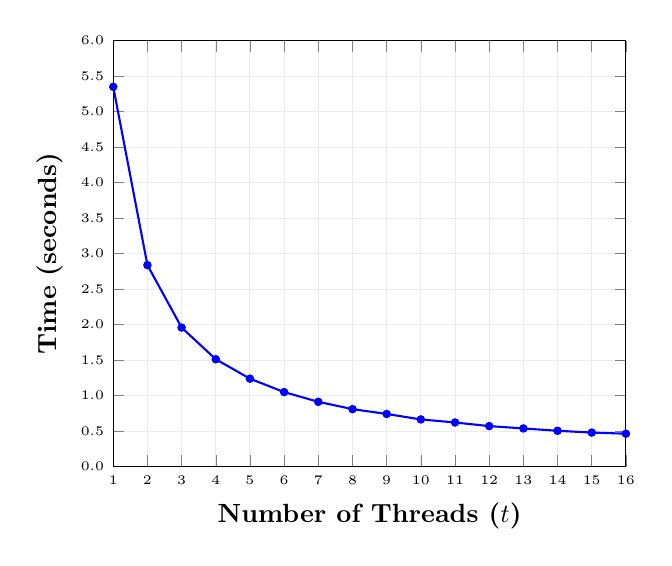
\begin{tikzpicture}[scale = 0.95]
\pgfplotsset{
    tick label style = {font=\tiny}
}
\begin{axis}[
    grid=both,
	grid style={gray!15},
    xlabel={\textbf{Number of Threads ($t$)}},
    ylabel={\textbf{Time (seconds)}},
    xmin=1, xmax=16,
    ymin=0.0, ymax=6.0,
    xtick distance=1,
    ytick distance=0.5,
    xmajorgrids=true,ymajorgrids=true,
    every axis plot/.append style={thick},
    y tick label style={/pgf/number format/.cd,fixed,fixed zerofill,precision=1,/tikz/.cd}
]
\addplot[color=blue, mark=*, mark options={scale=0.6}]
    coordinates {(1,5.350)(2,2.838)(3,1.958)(4,1.512)(5,1.238)(6,1.049)(7,0.912)(8,0.809)(9,0.741)(10,0.664)(11,0.621)(12,0.570)(13,0.537)(14,0.504)(15,0.479)(16,0.463)};
\end{axis}
\end{tikzpicture}}
  \captionof{figure}{Time (seconds) against Number of Threads for $d=1000, p=0.05, t=\{1,...,16\}$}
        \label{fig:TimeFixProb}
\end{minipage}\hspace{1.5cm}
\begin{minipage}[t]{0.55\textwidth}
As the number of threads increase from 1 to 16, the resulting execution time decreases in smaller intervals (referred to as ``diminishing returns'' \cite{padua2011}) which seems to show accordance with Amdahl's Law. For the fixed problem size there is indeed a fixed sequential overhead of thread creation, dividing cells between threads and so on, which is a limiting factor on the speedup obtained. Later experiments (e.g Appendix \ref{apdx:dimtime}) show that \textit{larger problem sizes} can produce larger speedup and efficiency values, which also confirms Gustafson's Law \cite{gustafson1988}. In other words, both Laws are correct but Amdahl considers a fixed size problem whereas Gustafson acknowledges that problem sizes usually increase with the number of processors available.
\end{minipage}
\\
\\
\\
As the matrix is subdivided into more parts, it seems that increasing the parallel part of the problem positively impacts the runtime, as \textsl{Balena} can schedule each thread on a separate core all the way up to $t=16$. See Appendix \ref{apdx:basicscaletests} for raw data. \textbf{Using the raw times calculated above, a graph of speedup and efficiency can be plotted.}
\\
\\
\\
\hspace{-0.5cm}\begin{minipage}[t]{0.4\textwidth}
  \centering\raisebox{\dimexpr \topskip-\height}{%
  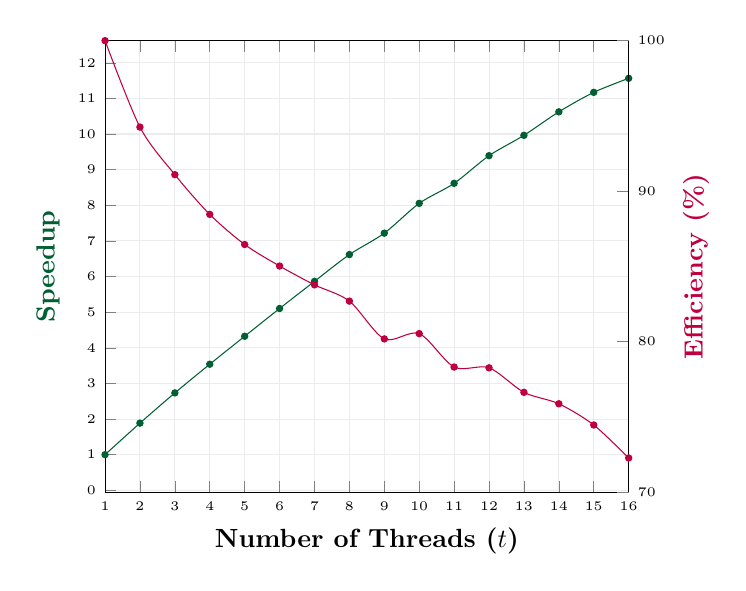
\begin{tikzpicture}[scale = 0.95]
\pgfplotsset{
	width=7cm,compat=1.3,tick label style = {font=\tiny}
}
  \begin{axis}[
    scale only axis,
    grid=both,
	grid style={gray!15},
    xmin=1, xmax=16,
    xtick distance=1,
    ytick distance=1,
    axis y line*=left,
    xlabel={\textbf{Number of Threads ($t$)}},
    ylabel={\textbf{\textcolor{forestgreen}{Speedup}}}]
  \addplot[smooth,mark=*, color=forestgreen,mark options={scale=0.6}]
  coordinates{
    (1,1)(2,1.885247827)(3,2.733015495)(4,3.538580247)(5,4.322919472)(6,5.102034329)(7,5.864450128)(8,6.616240725)(9,7.217176259)(10,8.053687908)(11,8.615673645)(12,9.39204213)(13,9.963376785)(14,10.62276638)(15,11.16979819)(16,11.56412104)
	};
  \end{axis}
  
  \begin{axis}[
    scale only axis,
   	ymin=70, ymax=100,
   	ytick distance=10.0,
    axis y line*=right,
    axis x line=none,
    xmin=1, xmax=16,
    ylabel={\textbf{\textcolor{purple}{Efficiency (\%)}}}]
    \addplot[smooth,mark=*, color=purple,mark options={scale=0.6}]
  coordinates{
    (1,100.00)(2,94.26)(3,91.10)(4,88.46)(5,86.46)(6,85.03)(7,83.78)(8,82.70)(9,80.19)(10,80.54)(11,78.32)(12,78.27)(13,76.64)(14,75.88)(15,74.47)(16,72.28)
	};
  \end{axis}
\end{tikzpicture}}
  \captionof{figure}{Speedup and Efficiency (\%) against Number of Threads for $d=1000, p=0.05, t=\{1,...,16\}$}
        \label{fig:SpeedupFixProb}
\end{minipage}\hspace{2.5cm}
\begin{minipage}[t]{0.45\textwidth}
Results show that for a fixed matrix size, the speedup values were almost linear with $t$. As more threads are added, more can be done in parallel across $t$ cores (scheduling 1 thread per core), which results in increased speedup values. As speedup values increase in a sub linear fashion, there is actually a decrease in efficiency from 100.00\% to 72.28\%. This can be attributed to the increase in scheduling overhead managing multiple threads - overall utilisation of the hardware is not as efficient as a larger fraction of time is spent scheduling than doing computation when $t$ increases. See Appendix \ref{apdx:basicscaletests} for raw data.
\end{minipage}


\hspace{-0.5cm}\begin{minipage}[t]{0.4\textwidth}
  \centering\raisebox{\dimexpr \topskip-\height}{%
  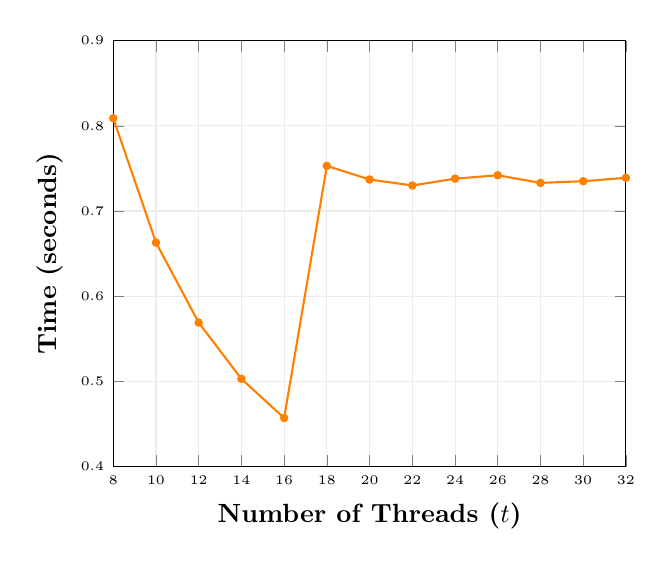
\begin{tikzpicture}[scale = 0.95]
\pgfplotsset{
    tick label style = {font=\tiny}
}
\begin{axis}[
    grid=both,
	grid style={gray!15},
    xlabel={\textbf{Number of Threads ($t$)}},
    ylabel={\textbf{Time (seconds)}},
    xmin=8, xmax=32,
    ymin=0.4, ymax=0.9,
    xtick distance=2,
    ytick distance=0.1,
    xmajorgrids=true,ymajorgrids=true,
    every axis plot/.append style={thick},
    y tick label style={/pgf/number format/.cd,fixed,fixed zerofill,precision=1,/tikz/.cd}
]
\addplot[color=orange, mark=*, mark options={scale=0.6}]
    coordinates {
    (8,0.809)(10,0.663)(12,0.569)(14,0.503)(16,0.457)(18,0.753)(20,0.737)(22,0.730)(24,0.738)(26,0.742)(28,0.733)(30,0.735)(32,0.739)
    };    
\end{axis}
\end{tikzpicture}}
  \captionof{figure}{Time (seconds) against Number of Threads for $d=1000, p=0.05, t=\{8,...,32\}$}
        \label{fig:TimeFixProbExt}
\end{minipage}\hspace{1.5cm}
\begin{minipage}[t]{0.55\textwidth}
\textsl{Balena} has 16 cores, so whilst creating more threads than this is possible, it means that there is a visible cost in terms of scheduling and management that causes the speedup and efficiency values to decrease. By increasing the value of $t$ beyond the number of cores available, there is a clear overhead in scheduling and waiting for idle threads to complete. The problem can't be as efficiently parallelised as before when $t>16$ because there are simply not enough cores to run 1 thread per core. This confirms the reason behind the abrupt increase in execution time observed when $t=18$ and above using the same size matrix with the same initial values as in the previous experiment using $t=\{1,...,16\}$. See Appendix \ref{apdx:cliff} for raw data.
\end{minipage}
\\
\\
\\
This cut-off point of $t=16$ is hardware specific to \textsl{Balena}, but the same pattern would be observed on any general shared memory multicore architecture - with $n$ cores, using a value $t > n$ causes the problem to be divided in a way that does not minimise the parallel fraction of the total runtime.  \textbf{Using the raw times calculated above, a graph of speedup and efficiency can be plotted.}
\\
\\
\hspace{-0.5cm}\begin{minipage}[t]{0.4\textwidth}
  \centering\raisebox{\dimexpr \topskip-\height}{%
  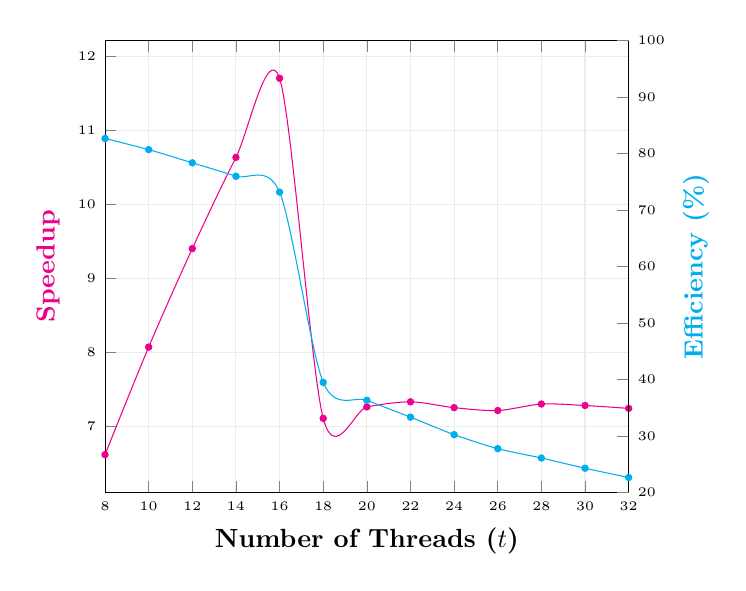
\begin{tikzpicture}[scale = 0.95]
\pgfplotsset{
	width=7cm,compat=1.3,tick label style = {font=\tiny}
}
  \begin{axis}[
    scale only axis,
    grid=both,
	grid style={gray!15},
    xmin=8, xmax=32,
    xtick distance=2,
    ytick distance=1,
    axis y line*=left,
    xlabel={\textbf{Number of Threads ($t$)}},
    ylabel={\textbf{\textcolor{magenta}{Speedup}}}]
  \addplot[smooth,mark=*, color=magenta,mark options={scale=0.6}]
  coordinates{
    (8,6.614)(10,8.070)(12,9.403)(14,10.637)(16,11.708)(18,7.105)(20,7.260)(22,7.329)(24,7.250)(26,7.211)(28,7.299)(30,7.279)(32,7.240)     
	};
  \end{axis}
  
  \begin{axis}[
    scale only axis,
   	ymin=20, ymax=100,
   	ytick distance=10.0,
    axis y line*=right,
    axis x line=none,
    xmin=8, xmax=32,
    ylabel={\textbf{\textcolor{cyan}{Efficiency (\%)}}}]
    \addplot[smooth,mark=*, color=cyan,mark options={scale=0.6}]
  coordinates{
    (8,82.67)(10,80.70)(12,78.36)(14,75.98)(16,73.17)(18,39.47)(20,36.30)(22,33.31)(24,30.21)(26,27.73)(28,26.07)(30,24.26)(32,22.62)    
	};
  \end{axis}
\end{tikzpicture}}
  \captionof{figure}{Speedup and Efficiency (\%) against Number of Threads for $d=1000, p=0.05, t=\{8,...,32\}$}
        \label{fig:SpeedupFixProbeExt}
\end{minipage}\hspace{2.5cm}
\begin{minipage}[t]{0.45\textwidth}
From the 72.28\% efficiency observed at $t=16$, the value unsurprisingly decreases a substantial amount once $t$ is increased further due to the overhead of scheduling more threads than there are cores available for the process. If the algorithm itself allowed for $t > (d-2)^{2}$, then increasing the value of $t$ to a value much larger would eventually cause symptoms of thrashing \cite{denning1968} - the scheduling overhead would dwarf the overall computation time. Using Amdahl's reasoning, the maximum speedup value is $11.708$ so this follows that the sequential fraction of the program (and limiting factor on speedup for this fixed problem size) for $d=1000, p=0.05$ is $\frac{1}{11.708} \times \approx  8.5\%$. This sequential fraction limits the maximum attainable speedup no matter how many processors are used, which confirms Amdahl's Law. See Appendix \ref{apdx:cliff} for raw data.
\end{minipage}

{\color{darkpurple}
\subsubsection*{Changing the Precision $p$}}
The next scalability experiments observed the effects of keeping a fixed problem size and thread count, whilst varying the precision value $p$.  It was observed that precision values of $p>0.1$ do not reap a lot of benefits from the parallel approach, as the difference in execution time between using 1 thread compared to 8 threads is not significant until $p$ is set to a value less than 0.1 (Figure \ref{fig:PrecTime}).
\begin{figure}[H]
\centering
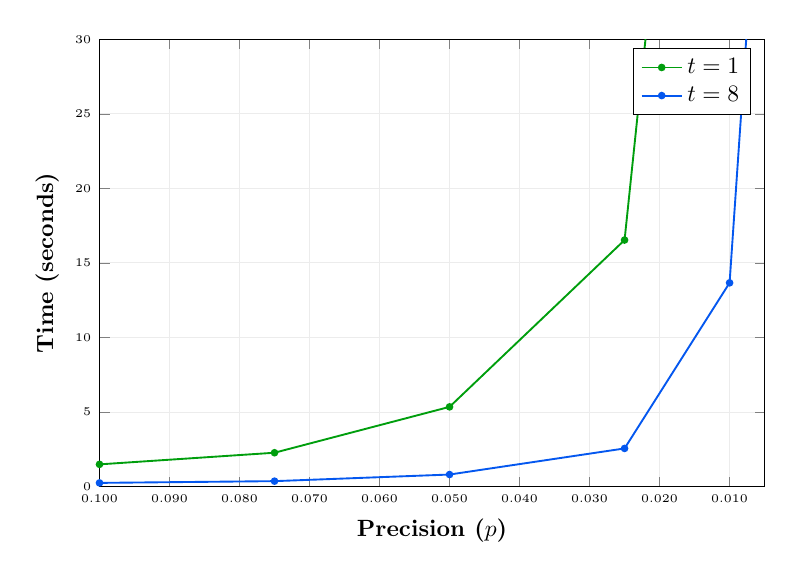
\begin{tikzpicture}[scale=0.85]
\pgfplotsset{
    tick label style = {font=\tiny}
}
\begin{axis}[
    grid=both,
    scaled y ticks = false,
    scaled x ticks = false,
   	width=0.95\textwidth,
    y post scale=0.8,
	grid style={gray!15},
    xlabel={\textbf{Precision ($p$)}},
    ylabel={\textbf{Time (seconds)}},
    x dir=reverse,
    xmin=0.005, xmax=0.1,
    ymin=0, ymax=30,
    xtick distance=0.01,
    ytick distance=5,
    xmajorgrids=true,ymajorgrids=true,
    every axis plot/.append style={thick},
    x tick label style={/pgf/number format/.cd,fixed,fixed zerofill,precision=3,/tikz/.cd}
]
\addplot[color=apple, mark=*, mark options={scale=0.6}]
    coordinates {
    (0.500,0.118)(0.400,0.151)(0.300,0.246)(0.200,0.519)(0.100,1.491)(0.075,2.271)(0.050,5.347)(0.025,16.536)(0.010,84.118)(0.005,295.644)    
    };
\addlegendentry{$t=1$}
\addplot[color=indigo, mark=*, mark options={scale=0.6}]
    coordinates {
    (0.500,0.034)(0.400,0.042)(0.300,0.054)(0.200,0.097)(0.100,0.248)(0.075,0.365)(0.050,0.808)(0.025,2.559)(0.010,13.666)(0.005,48.023)
    };
\addlegendentry{$t=8$}
\end{axis}
\end{tikzpicture}
\caption{Time (seconds) against Precision ($p$) for $t=\{1,8\}$, $d=1000$, $p=\{0.1,...,0.005\}$}
        \label{fig:PrecTime}
\end{figure}
A greater value for the precision $p$ generally causes a larger number of iterations to be required for a matrix to be relaxed. This means (for $t=8$ specifically) an increased fraction of the total runtime is spent by the threads themselves doing computations, which as seen before in Figure \ref{fig:SpeedupFixProb} allows more of the total program time to be executed in parallel across $t$ cores where $t\leq16$. As a consequence, there is a reduction in total execution time and an increase in speedup and efficiency values for a fixed problem size when the value of $p$ is reduced below 0.1. By increasing the thread count such that $8<t\leq16$, the same trend is observed, but overall runtimes are significantly reduced as $p$ is decreased below 0.1 at larger fixed values of $t$ within these limits. As before, this limit of $t\leq16$ is required for this pattern to be observed due to the specific architecture of \textsl{Balena}. This general pattern would be observed until $t=n$ for any shared memory architecture with $n$ cores. It must be noted that using very small precision values (e.g. $p<0.001$) could potentially lead to a number of iterations so large that \textsl{Balena} ``times out''. Furthermore, some combinations of initial matrix values may never terminate given this value if averages never converge. See Appendix \ref{apdx:prectests} for raw data.

\newpage
{\color{darkindigo}
\subsection{Varying the Matrix Dimension $d$}}
The next scalability tests involved varying the size of the matrix (size of problem) under a fixed thread count $t$, and constant fixed precision value $p$ (Figure \ref{fig:DimTime}) to see how this affected timings. The effect of an increase in matrix dimension from $d_1$ to $d_2$ is an increase in inner cell count by $(d_2-2)^2 - (d_1-2)^2$. In other words, the matrix dimension is not linear with the number of cells to relax.

As mentioned, Gustafson's Law states that the problem size scales with the number of processors $n$ which means that speedup is not bound by $n$ if larger problem sizes are considered \cite{gustafson1988}. The raw data in Appendix \ref{apdx:dimtime} shows this too - values for speedup and efficiency increase as the matrix dimension increases to larger sizes (scales). This is consistent with the graph of dimension $d$ against time for various fixed thread counts $t=\{1,4,8,16\}$ shown in Figure \ref{fig:DimTime} - larger fixed values of $t$ produced reduced execution times as the matrix size scales to larger values, with the difference in execution times in multithreaded configurations ($t\geq4$) becoming more pronounced as $d>2000$.  It is clear that dividing the matrix between threads is a much more scalable approach for larger matrix dimensions than simply executing the problem sequentially ($t=1$). For smaller problem sizes ($d<1000$) the difference in execution times between sequential and parallel implementations is far less pronounced, reinforcing the point that parallelism is only worth the initial overhead in thread management and work allocation if the problem is sufficiently large such that the initial parallel overheads do not dominate.

\begin{figure}[H]
\centering
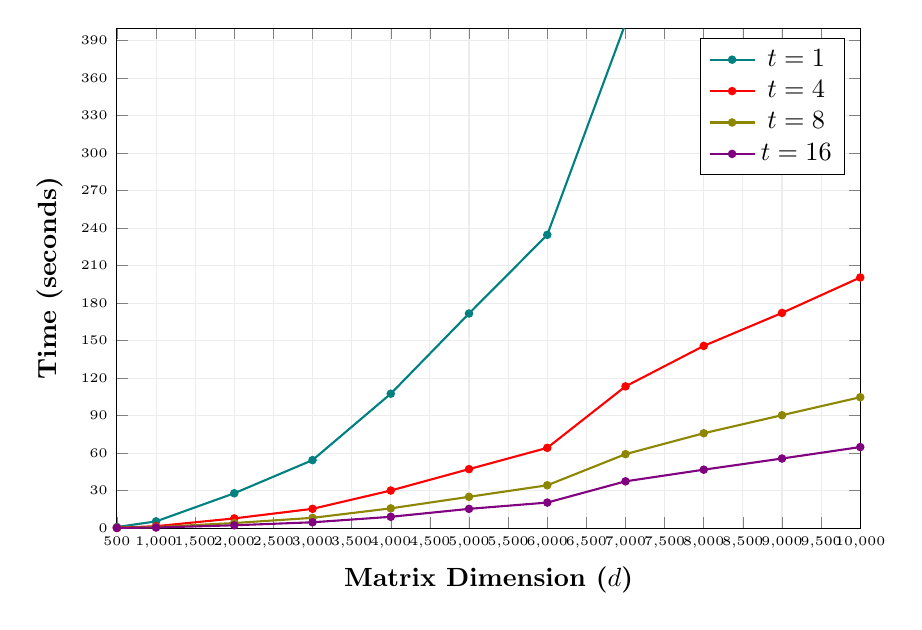
\begin{tikzpicture}[scale=0.95]
\pgfplotsset{
    tick label style = {font=\tiny}
}
\begin{axis}[
    grid=both,
    scaled y ticks = false,
    scaled x ticks = false,
   	width=0.95\textwidth,
    y post scale=0.8,
	grid style={gray!15},
    xlabel={\textbf{Matrix Dimension ($d$)}},
    ylabel={\textbf{Time (seconds)}},
    xmin=500, xmax=10000,
    ymin=0, ymax=400,
    xtick distance=500,
    ytick distance=30,
    xmajorgrids=true,ymajorgrids=true,
    every axis plot/.append style={thick}
]
\addplot[color=teal, mark=*, mark options={scale=0.6}]
    coordinates {
    (500,0.863)(1000,5.348)(2000,27.857)(3000,54.388)(4000,107.513)(5000,171.704)(6000,234.639)(7000,403.821)(8000,530.570)(9000,600)(10000,600)
    };
\addlegendentry{$t=1$}
\addplot[color=red, mark=*, mark options={scale=0.6}]
    coordinates {
    (500,0.249)(1000,1.513)(2000,7.754)(3000,15.416)(4000,30.051)(5000,47.180)(6000,64.201)(7000,113.377)(8000,145.767)(9000,172.161)(10000,200.526)
    };
\addlegendentry{$t=4$}
\addplot[color=olive, mark=*, mark options={scale=0.6}]
    coordinates {
    (500,0.144)(1000,0.808)(2000,4.048)(3000,8.203)(4000,15.789)(5000,25.027)(6000,34.260)(7000,59.162)(8000,75.899)(9000,90.340)(10000,104.710)
    };
\addlegendentry{$t=8$}
\addplot[color=violet, mark=*, mark options={scale=0.6}]
    coordinates {
    (500,0.097)(1000,0.456)(2000,2.250)(3000,4.641)(4000,9.027)(5000,15.384)(6000,20.415)(7000,37.415)(8000,46.737)(9000,55.666)(10000,64.832)
    };
\addlegendentry{$t=16$}
\end{axis}
\end{tikzpicture}
\caption{Time (seconds) against Matrix Dimension ($d$) for $d=\{500,...,10000\}, p=0.05, t=\{1,4,8,16\}$}
        \label{fig:DimTime}
\end{figure}

{\color{darkindigo}
\subsection{Further Speedup and Efficiency Calculations}
\label{sec:speedupeffic}}
The final scalability tests involved varying either the size of the matrix or the thread count $t$ whilst the other variable was fixed, with a constant fixed precision value $p$ to see how this affected speedup (Table \ref{tbl:Speedup}) and efficiency (Table \ref{tbl:Efficiency}) measurements. The below table cells have been coloured to indicate a particularly {\color{bad}{\textbf{low}}} or {\color{good!70!black}{\textbf{high}}} value of speedup or efficiency respectively, to make it easier to see the trend in how both values vary across varying matrix dimensions and thread counts. \textbf{Values have been calculated using the raw data in Appendix \ref{apdx:TimeTaken}.}

The speedup value using $n$ processors, $S_{n}$, is calculated as: $\dfrac{T_{s}+T_{p}}{T_{s}+\frac{T_{p}}{n}}$ where $T_{s}$ and $T_{p}$ account for the sequential and parallel execution times respectively \cite{gustafson1988}. The efficiency value using $n$ processors, $E_{n}$, is calculated as $\frac{S_{n}}{n}$. It is clear from these experiments that the value of $n$ which produces the largest $E_{n}$ (i.e. $n=1$) is not the same value of $n$ which produces the maximum $S_{n}$ (in this case $n=16$ using \textsl{Balena}). A careful consideration is needed by system designers depending on whether efficient use of hardware or reduced execution time is a priority.  The rationale behind the equal division of the matrix between threads, the thread pool approach and the minimised use of mutexes was to parallelise the problem as efficiently as possible. It is clear that this efficiency only shown in sufficiently large problem sizes.  Matrix dimensions of $d<100$ don't show much benefit from this effort. In fact, for $d\leq50, t\geq13$, $S_{n}<1$ which means the increase in overheads by increasing $t$ has actually made it quicker to solve this size of problem sequentially at precision $0.2$. For a fixed problem size there is indeed a natural limit on speedup, confirming Amdahl's Law.

It is only once the dimension $d$ increases beyond $1000\times1000$ that the benefits of parallelism are observed in the form of larger speedups whilst more threads are executed in parallel across $t$ cores (1 thread per core), confirming Gustafson's Law. For example, the greatest value of total speedup observed was 10.247 using 15 threads on a $15000\times15000$ matrix where the problem size is very large - $\sim \frac{(15000-2)^2}{15}$ cells are given to each thread to relax.

	\pgfplotstableset{
    color cells/.style={
        col sep=comma,
        font=\tiny,
        string type,
        trim cells=true,
        postproc cell content/.code={%
                \pgfkeysalso{@cell content=\rule{0cm}{0.4ex}\cellcolor{white!##1}\pgfmathtruncatemacro\number{##1}
                \ifnum\number>-1
                	\cellcolor{bad!50}
               \fi
                \ifnum\number>1
                	\cellcolor{badtoavg!50}
               \fi
               \ifnum\number>2
                	\cellcolor{avg}
               \fi
               \ifnum\number>3
                	\cellcolor{avgtogood}
               \fi
               \ifnum\number>7
               		\cellcolor{good}
               	\fi##1}%
                },
        columns/x/.style={
            column name={},
            fixed,
            postproc cell content/.code={}
        }
    }
}
\begin{table}[H]
\caption{Speedup across range of thread counts ($t=\{1,...,16\}$) and matrix dimensions ($d=\{10,...,20000\}$), with $p=0.2$.}\label{tbl:Speedup}
\centering
\pgfplotstabletypeset[color cells]{
x,10,50,100,250,500,1000,2500,5000,10000,15000,20000
1,1.000,1.000,1.000,1.000,1.000,1.000,1.000,1.000,1.000,1.000,1.000
2,1.000,1.000,1.250,1.556,1.793,1.790,1.844,1.903,1.840,1.891,1.929
3,1.000,1.000,1.667,2.000,2.476,2.495,2.646	,2.613,2.694,2.705,2.752
4,1.000,1.000,1.667,2.333,2.971,3.108,3.319,3.430,3.378,3.496,3.547
5,1.000,1.000,1.667,2.800,3.467,3.127,4.028,4.088,4.054,4.216,4.232
6,1.000,1.000,1.667,2.800,3.852,3.734,4.618,4.740,4.817,4.918,5.024
7,1.000,1.000,1.250,3.111,4.160,4.289,5.275,5.379,5.404,5.569,5.647
8,1.000,1.000,1.667,3.111,4.522,4.806,5.787,5.967,6.045,6.301,6.308
9,1.000,1.000,1.250,3.500,4.727,5.296,6.324,6.545,6.484,6.889,6.900
10,1.000,1.000,1.250,3.500,4.952,5.767,6.800,7.087,7.077,7.519,7.426
11,1.000,1.000,1.250,3.500,5.200,6.179,7.227,7.610,7.590,8.092,8.089
12,0.667,1.000,1.250,3.500,5.474,6.570,7.623,8.077,8.158,8.662,8.631
13,0.500,0.750,1.000,3.500,5.474,6.920,7.988,8.546,8.613,9.214,9.146
14,0.667,0.750,1.250,3.500,5.778,7.310,8.348,8.995,9.096,9.719,9.535
15,0.667,0.750,1.250,3.111,5.778,7.632,8.810,9.450,9.528,10.247,9.926
16,0.667,0.750,1.000,3.111,6.118,8.238,8.265,9.396,8.352,10.013,10.204
}
\end{table}

In support of Gustafson, the general trend seen in Table \ref{tbl:Efficiency} is that a growing problem size $d$ causes a general increase in efficiency.

\label{sec:effic}
	\pgfplotstableset{
    color cells/.style={
        col sep=comma,
        font=\tiny,
        string type,
        trim cells=true,
        postproc cell content/.code={%
                \pgfkeysalso{@cell content=\rule{0cm}{0.4ex}\cellcolor{white!##1}\pgfmathtruncatemacro\number{##1}
                \ifnum\number>-1
                	\cellcolor{bad!50}
               \fi
                \ifnum\number>25
                	\cellcolor{badtoavg!50}
               \fi
               \ifnum\number>50
                	\cellcolor{avg}
               \fi
               \ifnum\number>70
                	\cellcolor{avgtogood}
               \fi
               \ifnum\number>90
               		\cellcolor{good}
               	\fi##1}%
                },
        columns/x/.style={
            column name={},
            fixed,
            postproc cell content/.code={}
        }
    }
}
\begin{table}[H]
\caption{Efficiency (\%) across range of thread counts ($t=\{1,...,16\}$) and matrix dimensions ($d=\{10,...,20000\}$), with $p=0.2$.}\label{tbl:Efficiency}
\centering
\pgfplotstabletypeset[color cells]{
x,10,50,100,250,500,1000,2500,5000,10000,15000,20000
1,100.0,100.0,100.0,100.0,100.0,100.0,100.0,100.0,100.0,100.0,100.0
2,50.0,50.0,62.5,77.8,89.7,89.5,92.2,95.1,92.0,94.6,96.4
3,33.3,33.3,55.6,66.7,82.5,83.2,88.2,87.1,89.8,90.2,91.7
4,25.0,25.0,41.7,58.3,74.3,77.7,83.0,85.8,84.5,87.4,88.7
5,20.0,20.0,33.3,56.0,69.3,62.5,80.6,81.8,81.1,84.3,84.6
6,16.7,16.7,27.8,46.7,64.2,62.2,77.0,79.0,80.3,82.0,83.7
7,14.3,14.3,17.9,44.4,59.4,61.3,75.4,76.8,77.2,79.6,80.7
8,12.5,12.5,20.8,38.9,56.5,60.1,72.3,74.6,75.6,78.8,78.8
9,11.1,11.1,13.9,38.9,52.5,58.8,70.3,72.7,72.0,76.6,76.7
10,10.0,10.0,12.5,35.0,49.5,57.7,68.0,70.9,70.8,75.2,74.3
11,9.1,9.1,11.4,31.8,47.3,56.2,65.7,69.2,69.0,73.6,73.5
12,5.6,8.3,10.4,29.2,45.6,54.8,63.5,67.3,68.0,72.2,71.9
13,3.9,5.8,7.7,26.9,42.1,53.2,61.5,65.7,66.3,70.9,70.3
14,4.8,5.4,8.9,25.0,41.3,52.2,59.6,64.3,65.0,69.4,68.1
15,4.4,5.0,8.3,20.7,38.5,50.9,58.7,63.0,63.5,68.3,66.2
16,4.2,4.7,6.3,19.4,38.2,51.5,51.7,58.7,52.2,62.6,63.8
}
\end{table}
\footnotesize
\bibliography{Bibliography}
\normalsize
\begin{appendices}
{\color{indigo}
\section{Compiling and Running the \texttt{sharedrelax.c} program}
\label{apdx:runprog}}
Compiling the source code can be done with the gcc compiler (recommended). Once compiled into a binary file \texttt{sharedrelax}, the program is executable with customisable CLI parameters. Arguments are parsed with the getopt library\footnote{\url{https://www.gnu.org/software/libc/manual/html node/Getopt.html}}. An example compilation and run of the program might look like:	
\begin{lstlisting}[style=BashInputStyle]
    $		gcc -std=gnu99 -Wall -pthread sharedrelax.c -o sharedrelax
    $		./sharedrelax -d 1000 -t 16 -p 0.5 -v
\end{lstlisting}

The above runs the program using a $1000 \times 1000$ matrix with a precision of $0.5$ across $16$ threads, with verbose mode enabled.

\begin{table}[h]
\begin{center}
\caption{Program command line arguments.}
\label{tbl:CLIargs}
\begin{tabular}{|c|c|c|c|}
\hline
\textbf{Name} & \textbf{Description} & \textbf{Type} & \textbf{Default Value} \\
\hline
\texttt{d} & Matrix dimension & \texttt{Integer} & \texttt{50}\\
\texttt{p} & Precision & \texttt{Double} & \texttt{0.1}\\
\texttt{t} & Number of threads & \texttt{Integer} & \texttt{1}\\
\texttt{v} & Verbose mode & \texttt{Boolean} & \texttt{false}\\
\texttt{i} & Info mode & \texttt{Boolean} & \texttt{false}\\
\hline
\end{tabular}
\end{center}
\end{table}

Verbose mode (\texttt{-v}) prints details such as how workload is split between threads. Info mode (\texttt{-i}) just prints the state of the matrix after each iteration as well as the number of iterations it took to relax.

Other acceptable uses:
\begin{lstlisting}[style=BashInputStyle]
	$		./sharedrelax -d 15 -p 0.2 -t 1 -v
	$		./sharedrelax -d 15 -p 0.2 -t 1 -i
	$		./sharedrelax -d 125 -p 0.7 -t 5
	$		./sharedrelax -d 1000 -p 0.6 -t 20 -i
	$		./sharedrelax
\end{lstlisting}
A check is in place to validate whether $t > (d-2)^{2}$, as this is invalid in accordance with the way work is divided amongst threads using my approach. A minimum of 1 cell must be allocated to each thread.

\newpage
{\color{indigo}
\section{Testing Data and Results}
\label{apdx:testresults}}

{\color{darkindigo}
\subsection{Automated Correctness Testing for $t=\{2,...,50\}$, $d=\{10,...,1000\}$, $p=0.1$}
\tiny{\label{apdx:autocorrtests}
}
\color{black}
\begin{center}
\begin{tabular}{|l|l|l|l|l|}
\hline
\textbf{Dimension ($d$)} & \textbf{Precision ($p$)} & \textbf{Threads ($t$)} & \textbf{Repetitions} & \textbf{Result} \\
\hline
\texttt{10} & \texttt{0.1} & \texttt{2} & \texttt{100} & {\color{forestgreen!70}\texttt{Pass}}\\
\texttt{10} & \texttt{0.1} & \texttt{5} & \texttt{100} & {\color{forestgreen!70}\texttt{Pass}}\\
\texttt{10} & \texttt{0.1} & \texttt{10} & \texttt{100} & {\color{forestgreen!70}\texttt{Pass}}\\
\texttt{10} & \texttt{0.1} & \texttt{15} & \texttt{100} & {\color{forestgreen!70}\texttt{Pass}}\\
\texttt{10} & \texttt{0.1} & \texttt{20} & \texttt{100} & {\color{forestgreen!70}\texttt{Pass}}\\
\texttt{10} & \texttt{0.1} & \texttt{30} & \texttt{100} & {\color{forestgreen!70}\texttt{Pass}}\\
\texttt{10} & \texttt{0.1} & \texttt{50} & \texttt{100} & {\color{forestgreen!70}\texttt{Pass}}\\
\texttt{20} & \texttt{0.1} & \texttt{2} & \texttt{100} & {\color{forestgreen!70}\texttt{Pass}}\\
\texttt{20} & \texttt{0.1} & \texttt{5} & \texttt{100} & {\color{forestgreen!70}\texttt{Pass}}\\
\texttt{20} & \texttt{0.1} & \texttt{10} & \texttt{100} & {\color{forestgreen!70}\texttt{Pass}}\\
\texttt{20} & \texttt{0.1} & \texttt{15} & \texttt{100} & {\color{forestgreen!70}\texttt{Pass}}\\
\texttt{20} & \texttt{0.1} & \texttt{20} & \texttt{100} & {\color{forestgreen!70}\texttt{Pass}}\\
\texttt{20} & \texttt{0.1} & \texttt{30} & \texttt{100} & {\color{forestgreen!70}\texttt{Pass}}\\
\texttt{20} & \texttt{0.1} & \texttt{50} & \texttt{100} & {\color{forestgreen!70}\texttt{Pass}}\\
\texttt{50} & \texttt{0.1} & \texttt{2} & \texttt{100} & {\color{forestgreen!70}\texttt{Pass}}\\
\texttt{50} & \texttt{0.1} & \texttt{5} & \texttt{100} & {\color{forestgreen!70}\texttt{Pass}}\\
\texttt{50} & \texttt{0.1} & \texttt{10} & \texttt{100} & {\color{forestgreen!70}\texttt{Pass}}\\
\texttt{50} & \texttt{0.1} & \texttt{15} & \texttt{100} & {\color{forestgreen!70}\texttt{Pass}}\\
\texttt{50} & \texttt{0.1} & \texttt{20} & \texttt{100} & {\color{forestgreen!70}\texttt{Pass}}\\
\texttt{50} & \texttt{0.1} & \texttt{30} & \texttt{100} & {\color{forestgreen!70}\texttt{Pass}}\\
\texttt{50} & \texttt{0.1} & \texttt{50} & \texttt{100} & {\color{forestgreen!70}\texttt{Pass}}\\
\texttt{100} & \texttt{0.1} & \texttt{2} & \texttt{100} & {\color{forestgreen!70}\texttt{Pass}}\\
\texttt{100} & \texttt{0.1} & \texttt{5} & \texttt{100} & {\color{forestgreen!70}\texttt{Pass}}\\
\texttt{100} & \texttt{0.1} & \texttt{10} & \texttt{100} & {\color{forestgreen!70}\texttt{Pass}}\\
\texttt{100} & \texttt{0.1} & \texttt{15} & \texttt{100} & {\color{forestgreen!70}\texttt{Pass}}\\
\texttt{100} & \texttt{0.1} & \texttt{20} & \texttt{100} & {\color{forestgreen!70}\texttt{Pass}}\\
\texttt{100} & \texttt{0.1} & \texttt{30} & \texttt{100} & {\color{forestgreen!70}\texttt{Pass}}\\
\texttt{100} & \texttt{0.1} & \texttt{50} & \texttt{100} & {\color{forestgreen!70}\texttt{Pass}}\\
\texttt{200} & \texttt{0.1} & \texttt{2} & \texttt{100} & {\color{forestgreen!70}\texttt{Pass}}\\
\texttt{200} & \texttt{0.1} & \texttt{5} & \texttt{100} & {\color{forestgreen!70}\texttt{Pass}}\\
\texttt{200} & \texttt{0.1} & \texttt{10} & \texttt{100} & {\color{forestgreen!70}\texttt{Pass}}\\
\texttt{200} & \texttt{0.1} & \texttt{15} & \texttt{100} & {\color{forestgreen!70}\texttt{Pass}}\\
\texttt{200} & \texttt{0.1} & \texttt{20} & \texttt{100} & {\color{forestgreen!70}\texttt{Pass}}\\
\texttt{200} & \texttt{0.1} & \texttt{30} & \texttt{100} & {\color{forestgreen!70}\texttt{Pass}}\\
\texttt{200} & \texttt{0.1} & \texttt{50} & \texttt{100} & {\color{forestgreen!70}\texttt{Pass}}\\
\texttt{500} & \texttt{0.1} & \texttt{2} & \texttt{100} & {\color{forestgreen!70}\texttt{Pass}}\\
\texttt{500} & \texttt{0.1} & \texttt{5} & \texttt{100} & {\color{forestgreen!70}\texttt{Pass}}\\
\texttt{500} & \texttt{0.1} & \texttt{10} & \texttt{100} & {\color{forestgreen!70}\texttt{Pass}}\\
\texttt{500} & \texttt{0.1} & \texttt{15} & \texttt{100} & {\color{forestgreen!70}\texttt{Pass}}\\
\texttt{500} & \texttt{0.1} & \texttt{20} & \texttt{100} & {\color{forestgreen!70}\texttt{Pass}}\\
\texttt{500} & \texttt{0.1} & \texttt{30} & \texttt{100} & {\color{forestgreen!70}\texttt{Pass}}\\
\texttt{500} & \texttt{0.1} & \texttt{50} & \texttt{100} & {\color{forestgreen!70}\texttt{Pass}}\\
\texttt{1000} & \texttt{0.1} & \texttt{2} & \texttt{100} & {\color{forestgreen!70}\texttt{Pass}}\\
\texttt{1000} & \texttt{0.1} & \texttt{5} & \texttt{100} & {\color{forestgreen!70}\texttt{Pass}}\\
\texttt{1000} & \texttt{0.1} & \texttt{10} & \texttt{100} & {\color{forestgreen!70}\texttt{Pass}}\\
\texttt{1000} & \texttt{0.1} & \texttt{15} & \texttt{100} & {\color{forestgreen!70}\texttt{Pass}}\\
\texttt{1000} & \texttt{0.1} & \texttt{20} & \texttt{100} & {\color{forestgreen!70}\texttt{Pass}}\\
\texttt{1000} & \texttt{0.1} & \texttt{30} & \texttt{100} & {\color{forestgreen!70}\texttt{Pass}}\\
\texttt{1000} & \texttt{0.1} & \texttt{50} & \texttt{100} & {\color{forestgreen!70}\texttt{Pass}}\\
\hline
\end{tabular}
\end{center}}

\newpage
{\color{darkindigo}
\subsection{Time Taken (s), Speedup and Efficiency (\%) for for $t=\{1,...,16\}$, $d=1000$, $p=0.05$}
\footnotesize{\label{apdx:basicscaletests}
}
\color{black}
\begin{center}
\begin{tabular}{|l|l|l|l|}
\hline
Threads & Time (s) & Speedup & Efficiency (\%)\\
\hline
1 & 5.350 & 1.000 & 100.00\\
2 & 2.838 & 1.885 & 94.26\\
3 & 1.958 & 2.733 & 91.10\\
4 & 1.512 & 3.539 & 88.46\\
5 & 1.238 & 4.323 & 86.46\\
6 & 1.049 & 5.102 & 85.03\\
7 & 0.912 & 5.864 & 83.78\\
8 & 0.809 & 6.616 & 82.70\\
9 & 0.741 & 7.217 & 80.19\\
10 & 0.664 & 8.054 &  80.54\\
11 & 0.621 & 8.616 &  78.32\\
12 & 0.570 & 9.392 & 78.27\\
13 & 0.537 & 9.963 & 76.64\\
14 & 0.504 & 10.623 & 75.88\\
15 & 0.479 & 11.170 & 74.47\\
16 & 0.463 & 11.564 & 72.28\\
\hline
\end{tabular}
\end{center}}

{\color{darkindigo}
\subsection{Time Taken (s), Speedup and Efficiency (\%) for $t=\{8,...,32\}$, $d=1000$, $p=0.05$}
\footnotesize{\label{apdx:cliff}}
\color{black}
\begin{center}
\begin{tabular}{|l|l|l|l|}
\hline
Threads & Time (s) & Speedup & Efficiency (\%)\\
\hline
8 & 0.809 & 6.614 & 82.67\\
10 & 0.663 & 8.070 & 80.70\\
12 & 0.569 & 9.403 & 78.36\\
14 & 0.503 & 10.637 & 75.98\\
16 & 0.457 & 11.708 & 73.17\\
18 & 0.753 & 7.105 & 39.47\\
20 & 0.737 & 7.260 & 36.30\\
22 & 0.730 & 7.329 & 33.31\\
24 & 0.738 & 7.250 & 30.21\\
26 & 0.742 & 7.211 & 27.73\\
28 & 0.733 & 7.299 & 26.07\\
30 & 0.735 & 7.279 & 24.26\\
32 & 0.739 & 7.240 & 22.62\\
\hline
\end{tabular}
\end{center}}

\newpage
{\color{darkindigo}
\subsection{Time Taken (s) for $t=\{1, 4, 8, 16\}$, $d=\{500,...,10000\}$, $p=0.05$}
\footnotesize{\label{apdx:dimtime}}
\color{black}
\begin{center}
\begin{tabular}{|l|l|l|l|l|}
\hline
Dimension $d$ & Time (s) for $t=1$ & Time (s) for $t=4$ & Time (s) for $t=8$ & Time (s) for $t=16$\\
\hline
500 & 0.863 & 0.249 & 0.144 & 0.097\\
1000 & 5.348 & 1.513 & 0.808 & 0.456\\
2000 & 27.857 & 7.754 & 4.048 & 2.250\\
3000 & 54.388 & 15.416 & 8.203 & 4.641\\
4000 & 107.513 & 30.051 & 15.789 & 9.027\\
5000 & 171.704 & 47.180 & 25.027 & 15.384\\
6000 & 234.639 & 64.201 & 34.260 & 20.415\\
7000 & 403.821 & 113.377 & 59.162 & 37.415\\
8000 & 530.570 & 145.767 & 75.899 & 46.737\\
9000 & *Timeout* & 172.161 & 90.340 & 55.666\\
10000 & *Timeout* & 200.526 & 104.710 & 64.832\\
\hline
\end{tabular}
\end{center}}

{\normalsize From this, the speedup and efficiency can be calculated:}
\footnotesize{
\begin{center}
\begin{tabular}{|l|l|l|l|l|}
\hline
Dimension $d$ & Speedup for $t=1$ & Speedup for $t=4$ & Speedup for $t=8$ & Speedup for $t=16$\\
\hline
500 & 1.000 & 3.466 & 5.993 & 8.897\\
1000 & 1.000 & 3.535 & 6.619 & 11.728\\
2000 & 1.000 & 3.593 & 6.882 & 12.381\\
3000 & 1.000 & 3.528 & 6.630 & 11.719\\
4000 & 1.000 & 3.578 & 6.809 & 11.910\\
5000 & 1.000 & 3.639 & 6.861 & 11.161\\
6000 & 1.000 & 3.655 & 6.849 & 11.493\\
7000 & 1.000 & 3.562 & 6.826 & 10.793\\
8000 & 1.000 & 3.640 & 6.990 & 11.352\\
9000 & 1.000 & *N/A* & *N/A* & *N/A*\\
10000 & 1.000 & *N/A* & *N/A* & *N/A*\\
\hline
\end{tabular}
\end{center}}
\footnotesize{
\begin{center}
\begin{tabular}{|l|l|l|l|l|}
\hline
Dimension $d$ & Efficiency (\%) for $t=1$ & Efficiency (\%) for $t=4$ & Efficiency (\%) for $t=8$ & Efficiency (\%) for $t=16$\\
\hline
500 & 100.00 & 86.65 & 74.91 & 55.61\\
1000 & 100.00 & 88.37 & 82.74 & 73.30\\
2000 & 100.00 & 89.81 & 86.02 & 77.38\\
3000 & 100.00 & 88.20 & 82.88 & 73.24\\
4000 & 100.00 & 89.44 & 85.12 & 74.44\\
5000 & 100.00 & 90.98 & 85.76 & 69.76\\
6000 & 100.00 & 91.37 & 85.61 & 71.83\\
7000 & 100.00 & 89.04 & 85.32 & 67.46\\
8000 & 100.00 & 91.00 & 87.38 & 70.95\\
9000 & 100.00 & *N/A* & *N/A* & *N/A*\\
10000 & 100.00 & *N/A* & *N/A* & *N/A*\\
\hline
\end{tabular}
\end{center}}

\newpage
{\color{darkindigo}
\subsection{Time Taken (s) for $t=\{1,8\}$, $d=1000$, $p=\{0.5,...,0.005\}$}
\footnotesize{\label{apdx:prectests}}
\color{black}
\begin{center}
\begin{tabular}{|l|l|l|l|l|l|}
\hline
Precision $p$ & Iterations & Time (s) for $t=1$ & Time (s) for $t=8$ & Speedup & Efficiency (\%)\\
\hline
0.500 & 5 & 0.118 & 0.034 & 3.471 & 43.382\\
0.400 & 8 & 0.151 & 0.042 & 3.595 & 44.940\\
0.300 & 14 & 0.246 & 0.054 & 4.556 & 56.944\\
0.200 & 32 & 0.519 & 0.097 & 5.351 & 66.881\\
0.100 & 95 & 1.491 & 0.248 & 6.012 & 75.151\\
0.075 & 146 & 2.271 & 0.365 & 6.222 & 77.774\\
0.050 & 328 & 5.347 & 0.808 & 6.618 & 82.720\\
0.025 & 1030 & 16.536 & 2.559 & 6.462 & 80.774\\
0.010 & 5333 & 84.118 & 13.666 & 6.155 & 76.941\\
0.005 & 18313 & 295.644 & 48.023 & 6.156 & 76.954\\
\hline
\end{tabular}
\end{center}}

{\color{darkindigo}
\subsection{Time Taken (s) for $t=\{1,...,16\}$, $d=\{10,...,20000\}$, $p=0.2$}
\label{apdx:TimeTaken}}
\color{black}
	\pgfplotstableset{
    color cells/.style={
        col sep=comma,
        font=\footnotesize,
        string type,
        trim cells=true,
        postproc cell content/.code={%
                \pgfkeysalso{@cell content=\rule{0cm}{0.4ex}\cellcolor{white!##1}\pgfmathtruncatemacro\number{##1}
				\ifnum\number>-1
					\cellcolor{gray!25}
				 \fi
                ##1}%
                },
        columns/x/.style={
            column name={},
            fixed,
            postproc cell content/.code={}
        }
    }
}
\begin{table}[H]
\label{tbl:TimeTaken}
\centering
\pgfplotstabletypeset[color cells]{
x,10,50,100,250,500,1000,2500,5000,10000,15000,20000
1,0.002,0.003,0.005,0.028,0.104,0.519,3.339,14.733,62.029,175.406,265.536
2,0.002,0.003,0.004,0.018,0.058,0.290,1.811,7.743,33.704,92.738,137.685
3,0.002,0.003,0.003,0.014,0.042,0.208,1.262,5.639,23.026,64.837,96.477
4,0.002,0.003,0.003,0.012,0.035,0.167,1.006,4.295,18.360,50.168,74.867
5,0.002,0.003,0.003,0.010,0.030,0.166,0.829,3.604,15.299,41.600,62.742
6,0.002,0.003,0.003,0.010,0.027,0.139,0.723,3.108,12.877,35.664,52.856
7,0.002,0.003,0.004,0.009,0.025,0.121,0.633,2.739,11.478,31.496,47.020
8,0.002,0.003,0.003,0.009,0.023,0.108,0.577,2.469,10.262,27.839,42.098
9,0.002,0.003,0.004,0.008,0.022,0.098,0.528,2.251,9.567,25.460,38.484
10,0.002,0.003,0.004,0.008,0.021,0.090,0.491,2.079,8.765,23.329,35.758
11,0.002,0.003,0.004,0.008,0.020,0.084,0.462,1.936,8.173,21.676,32.826
12,0.003,0.003,0.004,0.008,0.019,0.079,0.438,1.824,7.603,20.249,30.764
13,0.004,0.004,0.005,0.008,0.019,0.075,0.418,1.724,7.202,19.037,29.033
14,0.003,0.004,0.004,0.008,0.018,0.071,0.400,1.638,6.819,18.048,27.848
15,0.003,0.004,0.004,0.009,0.018,0.068,0.379,1.559,6.510,17.117,26.751
16,0.003,0.004,0.005,0.009,0.017,0.063,0.404,1.568,7.427,17.518,26.022
}
\end{table}

{\normalsize Calculated speedup and efficiency values using this data can be seen in Section \ref{sec:speedupeffic}.}

\newpage
{\color{indigo}
\section{Automated Correctness Test Script}
\label{apdx:correctnesstest}}
\begin{minted}{bash}
#!/bin/bash

# Initialise variables
prec=0.1
repeat=100
nthreads=(2 5 10 15 20 30 50)
dims=(10 20 50 100 200 500 1000)
pass=1

for dim in "${dims[@]}"
do
    # Set expected output for current dimension (using t=1 as benchmark)
    ./sharedrelax -d $dim -t 1 -p $prec -i > in.txt

    # Check output matched by increasing number of threads
    for tcount in "${nthreads[@]}"
    do
        # Repeat each test to ensure some confidence in reproducibility
        for (( i=1; i<=$repeat; i++ )) 
        do  
            ./sharedrelax -d $dim -t $tcount -p $prec -i > out.txt

            # If files differ, failure!
            if [[ $(diff in.txt out.txt) ]]; then 
                pass=0
                echo "FAILED TEST for d=$dim, t=$tcount"
            fi
        done
        # Else if no trials fail, print success for this test case
        if [ "$pass" -eq "1" ]; then
            echo "PASSED TEST for d=$dim, t=$tcount"
        fi
    done
done

if [ "$pass" -eq "1" ]; then
   echo "All passed.";
   exit;
fi
\end{minted}

\end{appendices}
\end{document}